\documentclass[a4paper,14pt]{extarticle}

\usepackage[utf8x]{inputenc}
\usepackage[T1]{fontenc}
\usepackage[russian]{babel}
\usepackage{hyperref}
\usepackage{indentfirst}
\usepackage{here}
\usepackage{array}
\usepackage{graphicx}
\usepackage{grffile}
\usepackage{caption}
\usepackage{subcaption}
\usepackage{chngcntr}
\usepackage{amsmath}
\usepackage{amssymb}
\usepackage[left=2cm,right=2cm,top=2cm,bottom=2cm,bindingoffset=0cm]{geometry}
\usepackage{multicol}
\usepackage{multirow}
\usepackage{titlesec}
\usepackage{listings}
\usepackage{listingsutf8}
\usepackage{color}
\usepackage{enumitem}
\usepackage{cmap}
\usepackage{titlesec}

\definecolor{green}{rgb}{0,0.6,0}
\definecolor{gray}{rgb}{0.5,0.5,0.5}
\definecolor{purple}{rgb}{0.58,0,0.82}

\lstdefinelanguage{none}{}

\lstset{
	language={C++},
	inputpath={../},
	backgroundcolor=\color{white},
	commentstyle=\color{green},
	keywordstyle=\color{blue},
	numberstyle=\color{gray}\scriptsize\ttfamily,
	stringstyle=\color{purple},
	basicstyle=\lst@ifdisplaystyle\footnotesize\fi\ttfamily,
	breakatwhitespace=false,
	breaklines=true,
	captionpos=b,
	keepspaces=true,
	numbers=left,
	numbersep=5pt,
	showspaces=false,
	showstringspaces=false,
	showtabs=false,
	tabsize=4,
	frame=single,
	morekeywords={NULL, DWORD, WINAPI, HANDLE, STARTUPINFO, BYTE, LPSTR, SOCKET, WSADATA, TCHAR, LPCTSTR, LPOVERLAPPED, WSABUF, SECURITY_ATTRIBUTES, SECURITY_DESCRIPTOR, TRUE, FALSE, PROCESS_INFORMATION, PIPE_UNLIMITED_INSTANCES, LPVOID, sockaddr_in},
	deletekeywords={error},
	alsoletter={_},
	sensitive=true,
	extendedchars=false,
	columns=fullflexible,
	inputencoding=utf8/cp1251,
	literate=%
		{~}{{\raise.25ex\hbox{$\mathtt{\sim}$}}}{1}%
		{-}{-}{1}
}

\makeatletter
\def\lst@outputspace{{\ }}
\makeatother

\renewcommand{\le}{\ensuremath{\leqslant}}
\renewcommand{\leq}{\ensuremath{\leqslant}}
\renewcommand{\ge}{\ensuremath{\geqslant}}
\renewcommand{\geq}{\ensuremath{\geqslant}}
\renewcommand{\epsilon}{\ensuremath{\varepsilon}}
\renewcommand{\phi}{\ensuremath{\varphi}}
\renewcommand{\thefigure}{\arabic{figure}}
\newcommand{\code}[1]{\lstinline|#1|}
\newcommand{\caret}{\^{}}
\newcommand{\ctrl}[1]{\^{}{#1}}
\newcommand{\listingwithoutput}[1]{
	\lstinputlisting[caption=\code{#1.cpp}]{src/#1/#1.cpp}
	Выполним программу \code{#1.exe}:
	\lstinputlisting[language=none]{logs/#1/#1.txt}
}

\titleformat*{\section}{\large\bfseries}
\titleformat*{\subsection}{\normalsize\bfseries}
\titleformat*{\subsubsection}{\normalsize\bfseries}
\titleformat*{\paragraph}{\normalsize\bfseries}
\titleformat*{\subparagraph}{\normalsize\bfseries}

\titlespacing{\section}{0em}{0.8em}{0.8em}

\counterwithin{figure}{section}
\counterwithin{equation}{section}
\counterwithin{table}{section}
\newcommand{\sign}[1][5cm]{\makebox[#1]{\hrulefill}}
\newcommand{\equipollence}{\quad\Leftrightarrow\quad}
\newcommand{\no}[1]{\overline{#1}}
\graphicspath{{../pics/}}
\captionsetup{justification=centering,margin=1cm}
\def\arraystretch{1.3}
\setlength\parindent{5ex}
\titlelabel{\thetitle.\quad}

\setitemize{topsep=0em, itemsep=0em}
\setenumerate{topsep=0em, itemsep=0em}

\begin{document}

\begin{titlepage}
\begin{center}
	Санкт-Петербургский Политехнический Университет Петра Великого\\[0.3cm]
	Институт компьютерных наук и технологий \\[0.3cm]
	Кафедра компьютерных систем и программных технологий\\[4cm]
	
	\textbf{ОТЧЕТ}\\ 
	\textbf{по лабораторной работе}\\[0.5cm]
	\textbf{<<Процессы и потоки в Windows>>}\\[0.1cm]
	Операционные системы\\[3.0cm]
\end{center}

\begin{flushright}
	\begin{minipage}{0.5\textwidth}
		\textbf{Работу выполнил студент}\\[3mm]
		группа 43501/3 \hfill Дьячков В.В.\\[5mm]
		\textbf{Работу принял преподаватель}\\[5mm]
		\sign[2cm] \hfill к.т.н., доц. Душутина Е.В. \\[5mm]
	\end{minipage}
\end{flushright}

\vfill

\begin{center}
	Санкт-Петербург\\[0.3cm]
	\the\year
\end{center}
\end{titlepage}

\addtocounter{page}{1}

\tableofcontents
\newpage

\section{Цели работы}

Изучение видов межпроцессного взаимодействия в ОС Windows.

\section{Программа работы}

\renewcommand{\labelenumii}{\theenumii}
\renewcommand{\theenumii}{\theenumi.\arabic{enumii}.}

\textbf{Порождение и запуск процессов}

\begin{enumerate}
	\item Неименованные каналы (pipe):
		\begin{enumerate}
			\item Создать клиент-серверное приложение, позволяющее набираемые символы в терминальном окне командной строки (сервер) отображать их в окно процесса-потомка (клиент).
			\item Создать эхо-сервер, взаимодействующий с клиентом посредством pipe.
		\end{enumerate}
	\item Именованные каналы (named pipe):
		\begin{enumerate}
			\item Реализовать между одним клиентом и сервером обмен данными, вводимыми с консоли на стороне клиента и возвращаемыми сервером обратно до получения команды exit.
			\item Реализовать между сервером и множеством клиентов обмен данными, вводимыми с консоли на стороне клиента и возвращаемыми сервером обратно до получения команды exit.
			\item Модифицировать приложение из предыдущего примера для сетевого обмена информацией.
		\end{enumerate}
	\item Сокеты (socket):
		\begin{enumerate}
			\item Реализовать программ локального и сетевую обмена с помощью сокетов с использованием потокового протокола с установлением соединения (TCP в стеке TCP/IP).
			\item Модифицировать программу для локального обмена с множеством клиентов и с доступом к общему ресурсу. Провести эксперимент с множеством клиентов при сетевом обмене, представить результаты для виртуальной и реальной сетей.
			\item Проанализировать пример применения сокетов (сетевой обмен «мгновенными» сообщениями).
			\item Привести примеры использования портов завершения. Привести пример приложения с большим количеством клиентов до 1000 (когда порты завершения оправданы), общее количество потоков не более 10.
			\item Реализовать обмен на основе UDP.
		\end{enumerate}
	\item Сигналы (signal):
		\begin{enumerate}
			\item Задать обработчик сигналов завершения для консольного приложения.
			\item Самостоятельно предложить собственную реализацию обработчика сигнала.
		\end{enumerate}
	\item Разделяемая память (file mapping):
		\begin{enumerate}
			\item Создать программу, в которой первый процесс генерирует случайное число и записывает его в буфер, доступный второму процессу, откуда он его и считывает с последующим выводом.
		\end{enumerate}
	\item Почтовые слоты (MailSlot):
		\begin{enumerate}
			\item Предложить собственную реализацию приложения, иллюстрирующую обмен информацией почтовыми слотами. Продемонстрировать возможность локального и удаленного доступа. Выполнить широковещательную передачу данных.
		\end{enumerate}
\end{enumerate}

\section{Используемые операционные системы}

Реальная система:
\begin{itemize}
	\item ОС: Windows 10 Pro
	\item Версия ОС: 1803 (сборка 17134.345)
	\item Процессор: Intel® Core™ i7-4800MQ CPU @ 2.70GHz × 8
	\item IP-адрес в локальной сети: \code{192.168.0.101}
\end{itemize}

\lstinputlisting[language=none]{logs/host_ipconfig.txt}

Для тестирования сетевого взаимодействия было решено использовать виртуальную машину. Для этого с сайта Oracle VM VirtualBox\footnote{\url{https://www.virtualbox.org/wiki/Downloads}} была загружена версия для ОС Windows. Затем с сайта Ubuntu\footnote{\url{https://www.microsoft.com/ru-ru/software-download/windows10}} был загружен \code{.iso} образ операционной системы Windows 10. 

После этого был создан экземпляр виртуальной машине, в качестве boot-образа был указан загруженный образ Windows. Наконец, ОС была установлена и настроена. Сводная информация:
\begin{itemize}
	\item ОС: Windows 10 Home
	\item Версия ОС: 1803 (сборка 17134.1)
	\item Процессор: Intel® Core™ i7-4800MQ CPU @ 2.70GHz × 8
	\item IP-адрес в локальной сети: \code{192.168.0.102}
\end{itemize}

\lstinputlisting[language=none]{logs/virtualbox_ipconfig.txt}

\section{Неименованные каналы}

Посредством pipe-канала можно передавать данные только между двумя процессами. В основе взаимодействия лежит так называемая файловая модель функционирования. Один из процессов создает канал, другой открывает его. После этого оба процесса могут передавать данные через канал в одну или обе стороны, используя для этого функции, предназначенные для работы с файлами, такие как \code{ReadFile()} и \code{WriteFile()}.

\paragraph{Задание.} Создать клиент-серверное приложение, позволяющее набираемые символы в терминальном окне командной строки (сервер) отображать их в окно процесса-потомка (клиент).

\lstinputlisting[caption=\code{pipe_terminal_master.cpp}]{src/pipe/terminal/master/master.cpp}

\lstinputlisting[caption=\code{pipe_terminal_slave.cpp}]{src/pipe/terminal/slave/slave.cpp}

\newpage

Запустим \code{pipe_terminal_master.exe}:

\lstinputlisting[language=none]{logs/pipe/terminal/master.txt}

\lstinputlisting[language=none]{logs/pipe/terminal/slave.txt}

Видно, что запуске сервера создается канал, после чего порождается процесс \code{pipe_terminal_slave.exe} в новом окне. Любые символы, которые пишем в окне сервера, моментально появляются в окне клиента. Это достигается за счет того, что при порождении процесса в структуре \code{STARTUPINFO} поле \code{hStdInput} было заменено на читающий дескриптор канала.

\paragraph{Задание.} Создать эхо-сервер, взаимодействующий с клиентом посредством pipe.

В программе используется передача дескрипторов через наследование. По причине того, что анонимный канал является полудуплексным, для организации эхо-сервера необходимо создавать 2 канала (для передачи от клиента-серверу и обратно). При этом ненужные дескрипторы каналов закрываются только на стороне сервера (т.к. клиент наследует 4 дескриптора, а явно мы передаем только 2 дескриптора).

\lstinputlisting[caption=\code{pipe_echo_server.cpp}]{src/pipe/echo/server/server.cpp}

\lstinputlisting[caption=\code{pipe_echo_client.cpp}]{src/pipe/echo/client/client.cpp}

Запустим \code{pipe_echo_server.exe}:

\lstinputlisting[language=none]{logs/pipe/echo/server.txt}

\lstinputlisting[language=none]{logs/pipe/echo/client.txt}

Сервер создает два набора каналов чтобы обеспечить дуплексный обмен данными. После этого порождает процесс \code{pipe_echo_client.exe} и ожидает запрос от клиента. Приняв запрос, сервер фиксирует событие и отправляет это же сообщение обратно клиенту. Обмен происходит 10 раз, после чего процесс завершается.

\section{Именованные каналы}

Именованные каналы являются дуплексными, ориентированы на обмен сообщениями и обеспечивают взаимодействие через сеть. Кроме того, один именованный канал может иметь несколько открытых дескрипторов. Обмен данными может быть синхронным и асинхронным.

\subsection{Работа с одним клиентом}

\paragraph{Задание.} Реализовать между одним клиентом и сервером обмен данными, вводимыми с консоли на стороне клиента и возвращаемыми сервером обратно до получения команды exit.

Программа-сервер (\code{named_pipe_echo_server}) создает именованный канал для двунаправленного использования и ожидает подключения программы-клиента (\code{named_pipe_terminal_slave}). После подключения клиента, сервер ожидает сообщения от него сообщений и отправляет их обратно.

\lstinputlisting[caption=\code{named_pipe_echo_server.cpp}]{src/named_pipe/echo/server/server.cpp}

\lstinputlisting[caption=\code{named_pipe_echo_client.cpp}]{src/named_pipe/echo/client/client.cpp}

\newpage

Запустим сначала программу-сервер, а затем с помощью программы-клиента подключимся к созданному каналу и отправим несколько сообщений.

\lstinputlisting[language=none]{logs/named_pipe/echo/server.txt}

\lstinputlisting[language=none]{logs/named_pipe/echo/client.txt}

Из результатов видно, что сервер успешно создал канал, к которому после этого подключился клиент. Клиент отправляет сообщения в именованный канал, а сервер читает их оттуда и отправляет обратно. При получении команды \code{exit} и сервер, и клиент завершают свою работу.

\subsection{Работа с множеством клиентами}

\paragraph{Задание.} Реализовать между сервером и множеством клиентов обмен данными, вводимыми с консоли на стороне клиента и возвращаемыми сервером обратно до получения команды \code{exit}. Обеспечить возможность сетевого обмена информацией.

Для того, чтобы реализовать возможность обмена данными сервером с несколькими клиентами, воспользуемся механизмом потоков. В цикле будет создаваться экземпляр именованного канала, после чего ожидать подключения клиента. После подключения очередного клиента будет создан поток для взаимодействия с клиентом. Основная программа перейдет к ожиданию нового клиента. Для возможности сетевого обмена предусмотрим в клиентской программе возможность задания IP-адреса сервера с помощью параметра командной строки.

\lstinputlisting[caption=\code{named_pipe_multiecho_server.cpp}]{src/named_pipe/multiecho/server/server.cpp}

\lstinputlisting[caption=\code{named_pipe_multiecho_client.cpp}]{src/named_pipe/multiecho/client/client.cpp}

Протестируем работу с множеством клиентов локально. Запустим сервер и несколько клиентских приложений:

\lstinputlisting[language=none]{logs/named_pipe/multiecho/server.txt}

\lstinputlisting[language=none]{logs/named_pipe/multiecho/client1.txt}

\lstinputlisting[language=none]{logs/named_pipe/multiecho/client2.txt}

Видно, что сервер создает свой поток для каждого клиента, за счет чего достигается возможность одновременной работы нескольких клиентов.

Протестировать использование именованных каналов по сети не удалось, т.к. не удалось подключиться к удаленному серверу. В процессе поиска причин была найдена заметка в документации MSDN\footnote{https://msdn.microsoft.com/en-us/library/windows/desktop/aa365146(v=vs.85).aspx}, в которой говорится, что начиная с Windows 10 версии 1709 (версия используемой ОС -- 1803), именованные каналы поддерживаются только внутри контейнера приложения, что, видимо, и стало причиной невозможности подключиться к удаленному именованному каналу.

\newpage

\section{Сокеты}

Возможность взаимодействия с другими системами обеспечивается в Windows поддержкой сокетов (sockets) Windows Sockets -- совместимого и почти точного аналога сокетов Berkeley Sockets, де-факто играющих роль промышленного стандарта. Winsock API разрабатывался как расширение Berkley Sockets API для среды Windows и поэтому поддерживается всеми системами Windows.

При разработке предусмотрим возможность задавать серверу порт, на котором необходимо прослушивать соединения, а клиенту -- адрес и порт сервера. Общие для приложений функции, такие как \code{recvLine()}, \code{sendn()} и др., вынесем в статическую библиотеку \code{socket_utils}.

\lstinputlisting[caption=\code{utils.h}]{src/socket/utils/utils.h}

\lstinputlisting[caption=\code{utils.cpp}]{src/socket/utils/utils.cpp}

\subsection{Работа с одним клиентом по TCP}

\paragraph{Задание.} Реализовать программ локального и сетевую обмена с помощью сокетов с использованием потокового протокола с установлением соединения (TCP в стеке TCP/IP).

Для работы с одним клиентом на сервере нет необходимости создавать потоки, поэтому после начала работы дождемся подключения клиента и будем обмениваться сообщениями только с ним. Сервер выступает в роли echo-сервера, то есть отправляет в ответ те данные, которые были получены от клиента.

\lstinputlisting[caption=\code{socket_echo_server.cpp}]{src/socket/echo_server/server.cpp}

\lstinputlisting[caption=\code{socket_tcp_client.cpp}]{src/socket/tcp_client/client.cpp}

Протестируем локальный обмен сообщениями: запустим сервер на порту 7500 и подключимся к нему с помощью клиентского приложения.

\lstinputlisting[language=none]{logs/socket/echo/server.txt}

\lstinputlisting[language=none]{logs/socket/echo/client.txt}

Видно, что клиент успешно подключился к локальному серверу и обменялся сообщениями. После получения и отправки сообщения \code{exit} и клиент, и север завершили свою работу.

Для тестирования взаимодействия по сети будем использовать систему Windows 10 Home, установленную на виртуальную машину VirtulBox. Запустим на виртуальной машине серверное приложение и подключимся к нему, запустив на хостовой машине клиентское приложение (в качестве параметров командной строки передадим IP и порт сервера):

\lstinputlisting[language=none]{logs/socket/echo/remote_server.txt}

\lstinputlisting[language=none]{logs/socket/echo/remote_client.txt}

Видно, что клиент успешно подключился к удаленному серверу и обменялся сообщениями. После получения и отправки сообщения \code{exit} и клиент, и север завершили свою работу.

\subsection{Работа с множеством клиентом по TCP}

\paragraph{Задание.} Модифицировать программу для локального обмена с множеством клиентов и с доступом к общему ресурсу. Провести эксперимент с множеством клиентов при сетевом обмене, представить результаты для виртуальной и реальной сетей.

Для обмена с множеством клиентом модифицируем программу: для каждого клиента будем создавать свой поток на сервере с которым и будем происходить обмен. Главный поток будет в вечном цикле устанавливать соединения с новыми клиентами и создавать потоки. Список активных сокетов будем держать в глобальном векторе. Для синхронизации доступа к общему ресурсу будем использовать мьютекс. Клиентское приложение при этом остается без изменений.

\lstinputlisting[caption=\code{socket_multiecho_server.cpp}]{src/socket/multiecho_server/server.cpp}

Протестируем локальный обмен сообщениями: запустим сервер на порту 7500 и подключимся к нему несколькими клиентами.

\lstinputlisting[language=none]{logs/socket/multiecho/server.txt}

\lstinputlisting[language=none]{logs/socket/multiecho/client1.txt}

\lstinputlisting[language=none]{logs/socket/multiecho/client2.txt}

Видно, что сервер после старта создал сокет, связал его с портом 7500 и перевел в состояние слушающего. После каждого соединения с клиентом сервер выводит список активных сокетов. Оба клиента отправили по несколько сообщений и сервер успешно ответил на них.

Протестируем сетевой обмен: запустим на виртуальной машине серверное приложение и подключимся к нему, запустив на хостовой машине несколько клиентских приложений (передадим им в качестве параметров IP и порт сервера):

\lstinputlisting[language=none]{logs/socket/multiecho/remote_server.txt}

\lstinputlisting[language=none]{logs/socket/multiecho/remote_client1.txt}

\lstinputlisting[language=none]{logs/socket/multiecho/remote_client2.txt}

Видно, что клиенты так же успешно подключились к удаленному серверу на виртуальной машине и обменялись с ним сообщениями. После получения сообщения \code{exit} и сервер, и клиент завершили свою работу.

\subsection{Обмен мгновенными сообщениями}

\paragraph{Задание.} Проанализировать пример применения сокетов (сетевой обмен <<мгновенными>> сообщениями).

Чтобы реализовать сетевой обмен мгновенными сообщениями, сделаем сервер интерактивным. Вместо того, чтобы отправить пришедшие данные клиенту, он будет считывать ответ с консоли и отправлять клиенту считанную строку. Для этого добавим две строки к \code{socket_multiecho_server.cpp}:

\lstinputlisting[caption=\code{socket_chat_server.cpp}, linerange={34-35}]{src/socket/chat_server/server.cpp}

Протестируем обмен с удаленным сервером:

\lstinputlisting[language=none]{logs/socket/chat/remote_server.txt}

\lstinputlisting[language=none]{logs/socket/chat/remote_client.txt}

Видно, что серверу был задан порт 8888, к которому и подключился клиент. На сервере необходимо было вводить ответ на каждое сообщение, который после этого отправлялся клиенту.

\subsection{Порты завершения}

Порты завершения ввода/вывода, поддерживаемые лишь на NT-платформах, объединяют в себе возможности перекрывающегося ввода/вывода и независимых потоков и используются чаще всего в серверных программах.

Портами завершения ввода/вывода предоставляют возможность создавать ограниченное количество серверных потоков в пуле потоков, имея очень большое количество дескрипторов именованных каналов (или сокетов). При этом дескрипторы не соединяются попарно с отдельными рабочими серверными потоками; серверный поток может обслуживать любой дескриптор, данные которого нуждаются в обработке.

\paragraph{Задание.} Привести примеры использования портов завершения. Привести пример приложения с большим количеством клиентов до 1000 (когда порты завершения оправданы), общее количество потоков не более 10.

Разработаем серверное приложение (echo-сервер), которое будет использовать порты завершения для обработки запросов. Для создания порта и присоединения к нему дескрипторов используется одна и та же функция -- \code{CreateCompletionPort()}. Порт завершения ввода/вывода представляет собой совокупность дескрипторов файлов (или сокетов), открытых в режиме \code{OVERLAPPED}.

Поток ожидает завершения перекрывающейся операции ввода/вывода, находящейся в очереди, не путем ожидания события, а путем вызова функции \code{GetQueueCompletionStatus()} с указанием порта завершения (completion port).

Общую концепцию работу сервера можно описать следующим образом:
\begin{enumerate}
	\item Задание параметров для слушающего сокета сервера;
	\item Создание порта завершения и связывание со слушающим сокетом;
	\item Неявное создание очереди для ожидания запросов от клиентов на соединение;
	\item Создание рабочих потоков для обслуживания сообщений от порта завершения;
	\item Бесконечный цикл для многократного обслуживания запросов от клиентов, в котором, происходит \code{accept()} клиентов; 
	\item В рабочих потоках использование порта завершения с сокетом клиента, получение сообщения от клиента, формирование ответа.
\end{enumerate}

\lstinputlisting[caption=\code{socket_completion_server.cpp}]{src/socket/completion_server/server.cpp}

Запустим серверное приложение \code{socket_completion_server.exe} и несколько клиентских приложений, в качестве которых будем использовать разработанную ранее программу \code{socket_tcp_client.exe}.

\lstinputlisting[language=none]{logs/socket/completion/server.txt}

\lstinputlisting[language=none]{logs/socket/completion/client1.txt}

\lstinputlisting[language=none]{logs/socket/completion/client2.txt}

Видно, что клиенты подключились к удаленному серверу и отправили ему несколько сообщений. Для клиентских приложений не было заметно отличий, хотя на сервере использовалась другая процедура обработки запросов -- порты завершения.

Протестируем возможность сервера, использующего порты завершения, работы с большим количеством клиентов. Для этого модифицируем клиентское приложение: сделаем его не интерактивным. После запуска приложение будет раз в секунду отправлять сообщение серверу, IP-адрес и порт которого, как и отправляемое сообщение, задаются через параметры командной строки.

\lstinputlisting[caption=\code{socket_tcp_spam_client.cpp}]{src/socket/tcp_spam_client/client.cpp}

Напишем пакетный файл (batch file, \code{.bat}), аналог bash-скрипта в UNIX, с помощью которого можно будет запускать нужное количество клиентов.

\lstinputlisting[language=none,caption=\code{run.bat}]{src/socket/tcp_spam_client/run.bat}

Скрипт будет принимать три аргумента -- IP-адрес и порт сервера, а также количество клиентских приложений, которое необходимо запустить.

Запустим на виртуальной машине серверное приложение, использующее порты завершения для обработки запросов. На хостовой машине для тестирования запустим скрипт, создав 5 клиентов: \code{run.bat 192.168.0.102 7500 5}.

\lstinputlisting[language=none]{logs/socket/completion/test.txt}

Видно, что к серверу подключились ровно 5 клиентов и начали отправлять сообщение <<Message form N>>, где N -- номер клиента.

Попробуем запустить скрипт, создав 1000 клиентов. Предварительно закомментируем на сервере отладочную печать чтобы снизить нагрузку. Будем фиксировать загрузку ЦП на стороне сервера.

\begin{figure}[H]
	\centering
	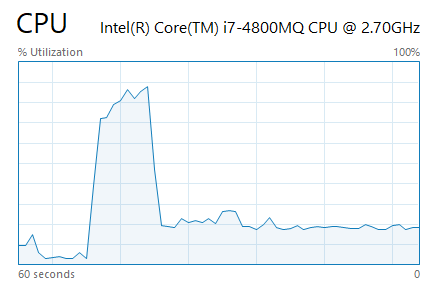
\includegraphics[width=0.7\linewidth]{1k_clients}
	\caption{Загрузка ЦП на сервере при подключении 1000 клиентов}
\end{figure}

Видно, что загрузка ЦП была близка к максимальной в самом начале работы -- установлении соединения с 1000 клиентов. После этого загрузка упала до 20\%, сервер при этом успешно отвечал на запросы клиентов.

\subsection{Работа с множеством клиентов по UDP}

\paragraph{Задание.} Реализовать обмен на основе UDP.

Реализуем обмен с множеством клиентом на основе UDP, то есть без установления соединения. Сервер, получив сообщение, сразу отсылает его обратно на адрес и порт отправителя.

\lstinputlisting[caption=\code{socket_udp_server.cpp}]{src/socket/udp_server/server.cpp}

\lstinputlisting[caption=\code{socket_udp_client.cpp}]{src/socket/udp_client/client.cpp}

Запустим серверное приложение на виртуальной машине, а клиентское -- на хостовой.

\lstinputlisting[language=none]{logs/socket/udp/remote_server.txt}

\lstinputlisting[language=none]{logs/socket/udp/remote_client.txt}

Видно, что клиент успешно отправил серверу несколько сообщений и завершился. Сервер при получении каждого сообщения выводит информацию об отправителе: IP-адрес и порт.

UDP работает быстрее чем TCP, потому что не устанавливает соединение, но он менее надежен и не гарантирует доставку пакетов и очередность их доставки.

\section{Сигналы}

Данное средство IPC в Windows не поддерживается. Однако, например, консольному приложению можно посылать сигналы \caret\code{C} и \caret\code{BREAK}. Система может посылать приложению сигналы: \caret\code{CLOSE_EVENT}, \caret\code{LOGOFF_EVENT} и \caret\code{SHUTDOWN_EVENT}, когда пользователь закрывает консоль, выходит из системы, или когда система завершается. По получению данных сигналов процесс может произвести корректное завершение.

\paragraph{Задание.} Задать обработчик сигналов завершения для консольного приложения.

Задать обработчик, перехватывающий сигналы \caret\code{C} и \caret\code{BREAK}. При этом обработчик смотрит, какой сигнал ему передан, и выводит его название. Для звуковой индикации работы приложение вызывает функцию \code{Beep()}. Данная функция воспроизводит звуковой сигнал через динамик консоли с разной частотой и длительностью, задаваемыми ей через параметры.

\lstinputlisting[caption=\code{signal_handler.cpp}]{src/signal/handler/handler.cpp}

Запустим \code{handler.exe} и попробуем отправить из консоли несколько сигналов:

\lstinputlisting[language=none]{logs/signal/handler.txt}

Видно, что приложение обработало несколько раз сигнал \caret\code{C}, но при получении сигнала \caret{\code{BREAK}} приложение было завершено (действие по умолчанию). Это произошло из-за того, что из функции обработчика было возвращено \code{FALSE} (сигнал не обработан) и обработкой сигнала занимался обработчик по умолчанию, который и завершил процесс.

\paragraph{Задание.} Самостоятельно предложить собственную реализацию обработчика сигнала.

Модифицируем программу: после получения сигнала \caret\code{C} приложение будет восстанавливать исходный обработчик сигнала. Для этого вызывается функция \code{SetConsoleCtrlHandler()} со вторым параметром \code{FALSE}.

\lstinputlisting[caption=\code{signal_multihandler.cpp}, linerange={9-10}]{src/signal/multihandler/multihandler.cpp}

Запустим \code{multihandler.exe} и попробуем отправить из консоли несколько сигналов:

\lstinputlisting[language=none]{logs/signal/multihandler.txt}

Видно, что после получения первого сигнала \caret\code{C} был установлен обработчик по умолчанию и после получения второго сигнала приложение было завершено.

Возможностей сигналов в Windows, по сравнению с UNIX, сильно меньше, но они могут быть полезны для консольных приложений.

\section{Разделяемая память}

Потоки одного процесса могут разделять общую память этого процесса. У каждого процесса -- свое изолированное адресное пространство. Кроме рассмотренных выше средств передачи информации между процессами или потоками разных процессов, одно из наиболее эффективных – использование общей памяти, доступ к которой обеспечивается со стороны каждого процесса. ОС Windows поддерживает такое средство, как именованная, совместно используемая память.

\paragraph{Задание.} Создать программу, в которой первый процесс генерирует случайное число и записывает его в буфер, доступный второму процессу, откуда он его и считывает с последующим выводом.

Создадим приложение \code{writer} (писатель), который будет генерировать случайные значения, и \code{reader} (читатель), который будет читать и выводить в консоль эти значения.

Для организации синхронизации доступа к памяти используется мьютекс. В первом процессе создается именованный мьютекс, который <<защищает>> критические участки кода, в данном случае -- запись в общую разделяемую память. Второй процесс открывает ранее созданный и именованный первым процессом мьютекс.

\lstinputlisting[caption=\code{shmem_writer.cpp}]{src/shmem/writer/writer.cpp}

\lstinputlisting[caption=\code{shmem_reader.cpp}]{src/shmem/reader/reader.cpp}

Запустим писателя и читателя:

\lstinputlisting[language=none]{logs/shmem/writer.txt}

\lstinputlisting[language=none]{logs/shmem/reader.txt}

Видно, что писатель генерировал случайные значения, а писатель их читал и выводил в консоль. За счет использования средств синхронизации была исключена ситуация <<гонок>> между процессами, система разделения доступа к памяти сработала правильно.

\section{Почтовые слоты}

MailSlot -- механизм синхронизации, иначе называемый <<почтовый ящик>>. Каждый слот реализуется как псевдофайл в оперативной памяти и содержит некоторое количество записей (<<сообщений>>), которые могут быть прочтены всеми компьютерами в сетевом домене. Общий размер данных не дможет превышать 64K. В отличие от дисковых файлов, файлы MailSlot временные. Когда все указатели на MailSlot закрываются, MailSlot и все данные, которые он содержит, удаляются.

\paragraph{Задание.} Предложить собственную реализацию приложения, иллюстрирующую обмен информацией почтовыми слотами. Продемонстрировать возможность локального и удаленного доступа. Выполнить широковещательную передачу данных.

Разработаем серверное и клиентское приложения. Сервер будет создавать MailSlot и в вечном цикле проверять его на наличие новых сообщений. При получении сообщения, сервер будет выводить его и количество полученных байт. Клиентское приложение будет работать в интерактивном режиме, читая из консоли сообщения, которые необходимо отправить серверу. Изначально предусмотрим возможность задания клиенту адреса сервера:
\begin{itemize}
	\item <<{\Large\code{.}}>> -- локальный сервер;
	\item <<\code{COMPUTER_NAME}>> -- удаленный сервер;
	\item <<\code{*}>> - широковещательная передача;
\end{itemize} 

\lstinputlisting[caption=\code{mailslot_server.cpp}]{src/mailslot/server/server.cpp}

\lstinputlisting[caption=\code{mailslot_client.cpp}]{src/mailslot/client/client.cpp}

Протестируем возможность локальной передачи:

\lstinputlisting[language=none]{logs/mailslot/server.txt}

\lstinputlisting[language=none]{logs/mailslot/client.txt}

Протестируем возможность удаленной передачи. Для этого запустим сервер на хостовой машине и клиента на виртуальной машине, передав ему имя компьютера:

\lstinputlisting[language=none]{logs/mailslot/remote_server.txt}

\lstinputlisting[language=none]{logs/mailslot/remote_client.txt}

Протестируем возможность широковещательной передачи. Для этого запустим локальный сервер и сервер на виртуальной машине. После этого запустим клиента, указав ему адрес сервера <<\code{*}>>:

\lstinputlisting[language=none]{logs/mailslot/broadcast_server1.txt}

\lstinputlisting[language=none]{logs/mailslot/broadcast_server2.txt}

\lstinputlisting[language=none]{logs/mailslot/broadcast_client.txt}

Видно, что оба сервера, находящиеся в одной сети с клиентом, получили широковещательные сообщения и завершились после получения сообщения \code{exit}.

\section{Выводы}

В процессе выполнения данной работы:

\begin{itemize}
	\item изучены различные типы средства межпроцессорного взаимодействия в Windows;
	\item рассмотрены возможности неименованных и именованных каналов;
	\item продемонстрированы возможности использования сигналов для консольного приложения; 
	\item рассмотрены почтовые слоты и разделяемая память как вид межпроцессного взаимодействия.
\end{itemize}

\section*{Список использованных источников}

\begin{enumerate}
	\item Душутина Е.В. - Системное программное обеспечение. Практические вопросы разработки системных приложений [Текст] -- 2016.
	\item Таненбаум Э. - Современные операционные системы [Текст] -- 2015.
	\item Named Pipe Instances / Microsoft Docs [Электронный ресурс]:\\
		{\small\url{https://docs.microsoft.com/en-us/windows/desktop/ipc/named-pipe-instances}} 
	\item Multithreaded Pipe Server / Microsoft Docs [Электронный ресурс]:\\
		{\small\url{https://docs.microsoft.com/en-us/windows/desktop/ipc/multithreaded-pipe-server}} 
	\item Порты завершения ввода/вывода / Системное программирование в среде Windows [Электронный ресурс]:\\
		{\small\url{https://it.wikireading.ru/1583}} 
\end{enumerate}

\end{document}
